\chapter{人脸检测算法}
\label{chap:facedetection}

人脸检测算法自上世纪以来已经被无数研究者探究过,检测的准确率也是逐年提高。在本系统中,我们需要的是一个能够优秀的处理大角度人脸、模糊人脸甚至部分被遮挡人脸的检测算法。在保证非常高的准确率的同时,该算法需要有非常快的执行速度,以适应同时处理大量图片的需求。



以CFDDB中的图片为标准,我们要求人脸检测算法需要在 定义的$recall\geq 80\%$的情况下,在一张Nvidia 1080 Ti显卡的支持下处理一张宽1600像素,高1200像素的图片的平均速度不超过\SI{500}{ms}。


\section{基于HAAR特征的级联分类器}

\subsection{概述}
HAAR特征在物体检测领域有着广泛的应用,在2001年,Paul Viola和Michael Jones在论文[9]中提出了使用HAAR特征来检测人脸的方法。这种方法的基本思想是在一系列含有人脸区域的正图像和不含人脸的负图像上训练训练一系列的分类器,然后将分类器级联组合,得到完成的人脸检测函数。在分类器的训练中,我们通过提取提取图\ref{fig:HAAR}所示的三种不同种类HAAR特征来判断一个特定的区域是否属于人脸区域。

\begin{figure}[!htp]
	\centering
	\subcaptionbox{边特征\label{fig:HAAR:A}}
	{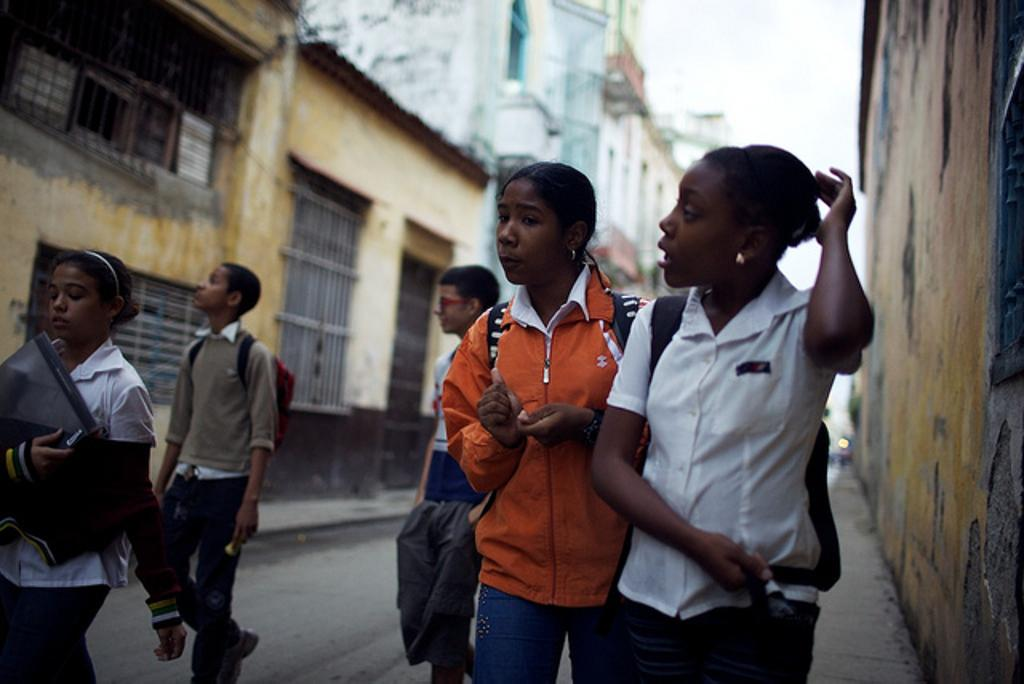
\includegraphics[height=3cm]{chap2/1.jpg}}
	\hspace{4em}
	\subcaptionbox{四矩形特征\label{fig:HAAR:B}}
	{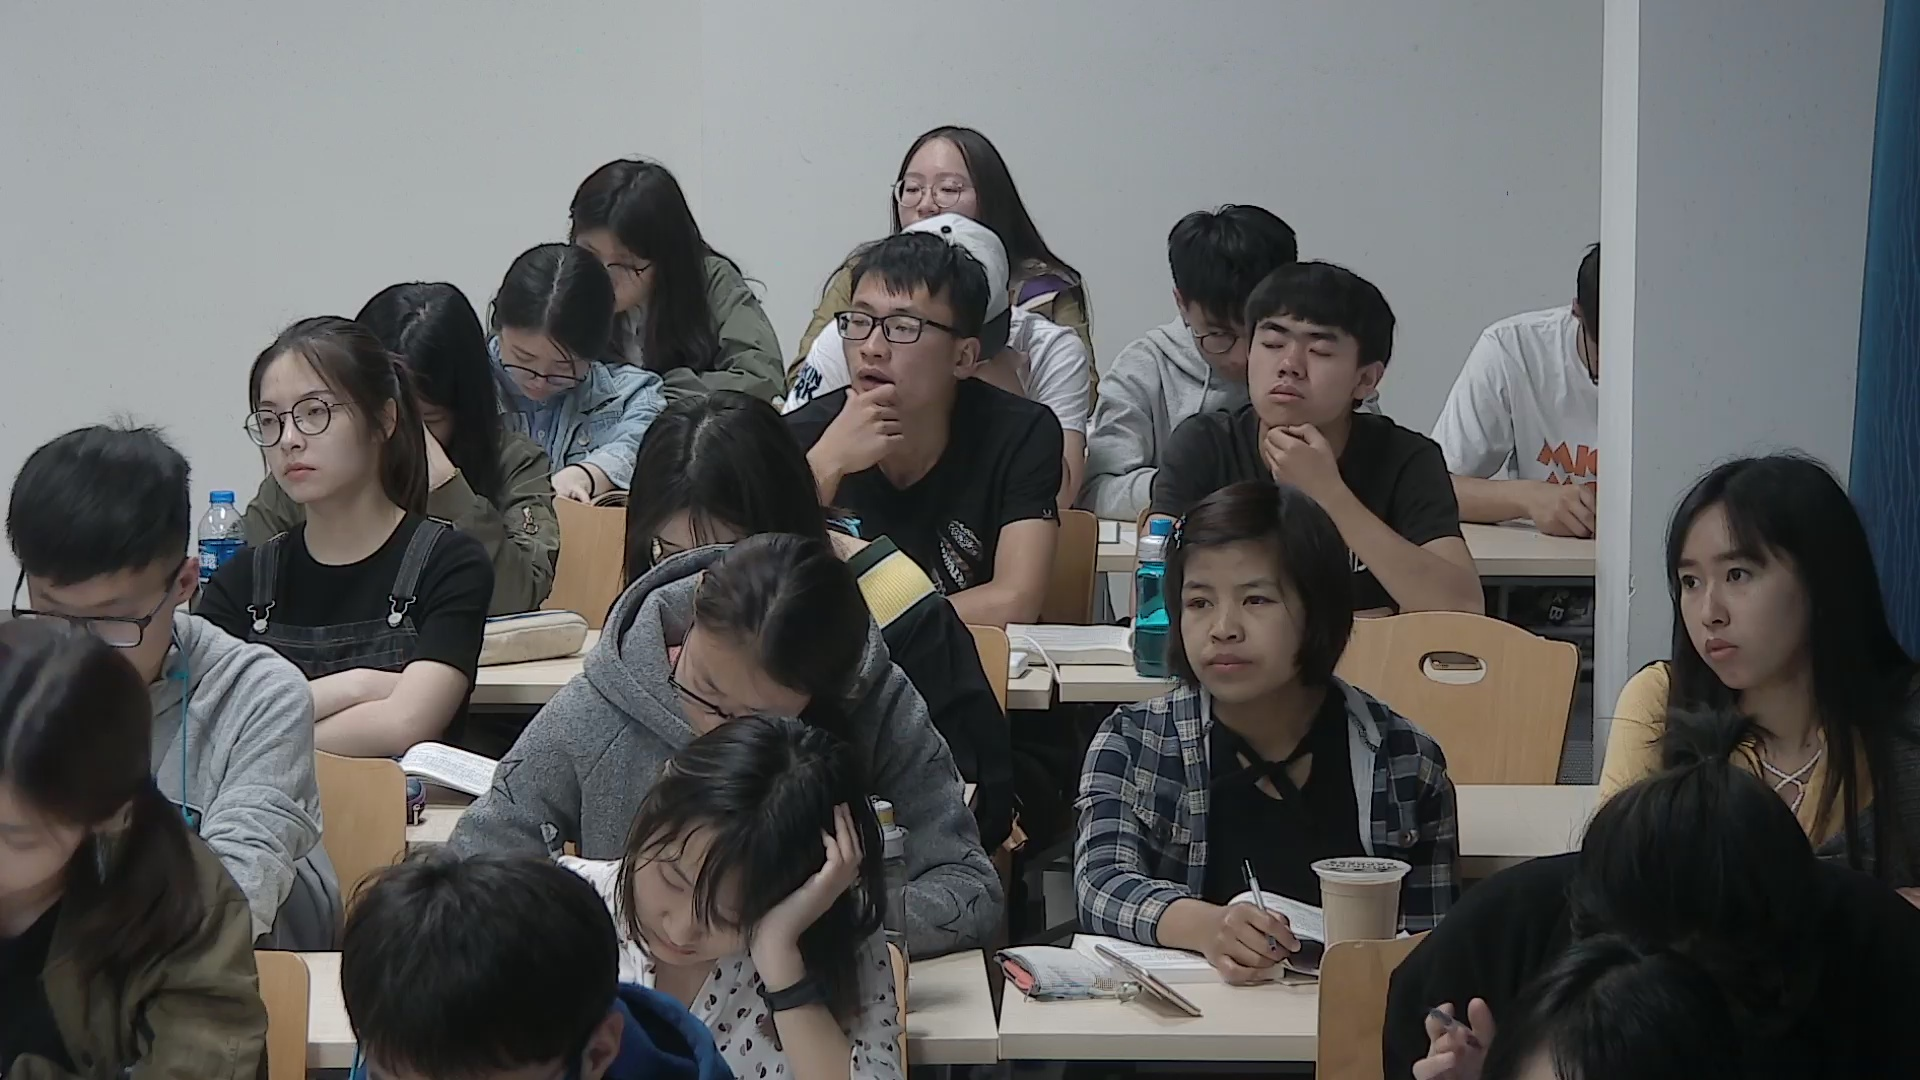
\includegraphics[height=3cm]{chap2/2.jpg}}
	\hspace{4em}
	\subcaptionbox{线特征\label{fig:HAAR:C}}
	{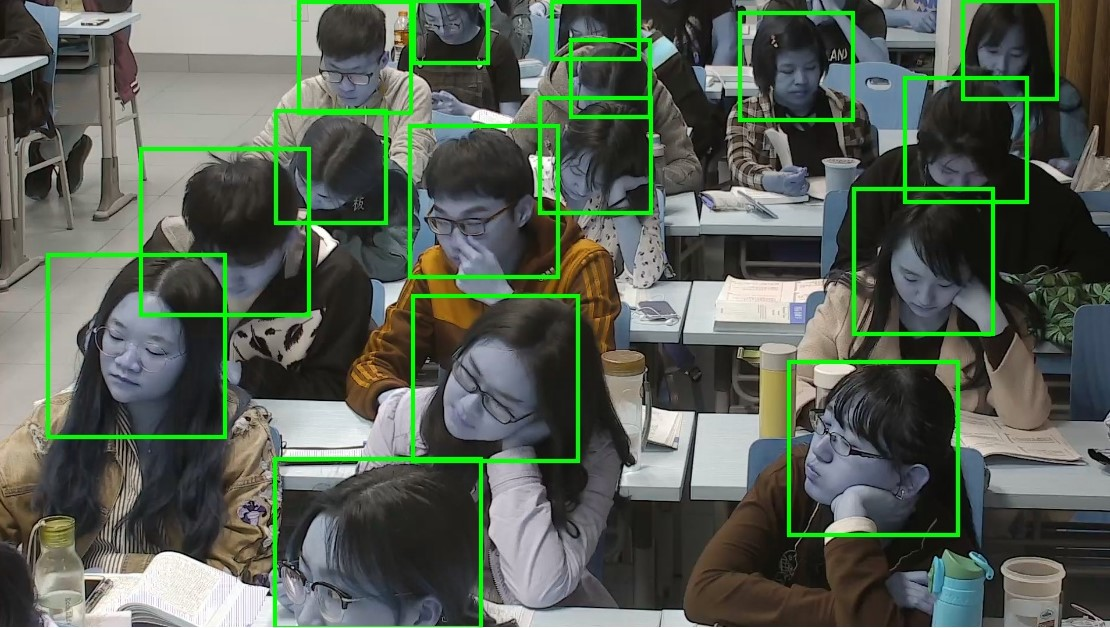
\includegraphics[height=3cm]{chap2/3.jpg}}
	\bicaption{三种HAAR特征}{Three HAAR features}
	\label{fig:HAAR}
\end{figure}

在提取特征前,需要将图像转化为灰度图。三种特征中,图\ref{fig:HAAR:A}的边特征和图\ref{fig:HAAR:C}的线特征在顺时针旋转90度之后提取的特征归为同类特征。特征值的是将某一个特征中黑色部分区域的灰度值之和减去白色区域灰度值之和得到的。

同一种类的特征区域的大小可以不同,提取特征的图片区域可以不同,这样就导致了即使是非常小的一张图片,其所能够提取到的HAAR特征也是非常多的。例如,在一张宽24像素,高24像素的图片中,可以提取的特征可以超过了16万种。如果选取所有的特征进行比对,那么所花费的计算代价是不可接受的。因此,必须对特征进行选择。

首先,对每个特征进行训练,让它可以在训练集上尽可能区分开有人脸的图片和没有人脸的图片。接着计算这个特征的错误率。在所有特征都训练完毕之后选取错误率最小的部分特征作为需要的特征保留。最后,将选取的特征加权求和,作为一个分类器使用。

根据论文[9]中的叙述,每一个特征单独的分类效果较差,但是将所有特征加权求和得到的分类器则非常强大。使用200特征则可达到$95\%$以上的准确率。论文中最终的分类器使用了约6000个特征,具有非常强大的检测能力。

然而,对于一张图片所有可能的区域计算6000个特征仍然是一件非常耗时的工作,对此,作者提出了使用级联分类器的方法来解决。所谓级联,就是将分类器串接起来,只有通过前面分类器检测的图片区域才会继续进行下一分类器的检测。在文章中,分类器共有38级,平均每个区域的识别所需要提取约10个特征。这样的方式极大的加快了分类器的处理速度。

\subsection{在CFDDB上的测试结果}

我们使用OpenCV预训练好的HAAR级联分类器[10]进行检测。这个分类器共有两个可变参数,minNeighbor和scaleFactor。其中minNeighbor表示构成人脸区域的相邻的小矩形个数,scaleFactor表示在两次相继的扫描中,搜索框的比例系数。为了更好的检测HAAR级联分类器的效果,我们选取了不同的minNeighbor和scaleFactor参数在CFDDB上进行了测试,表\ref{tab:haar}为测试结果:

\begin{table}[!hpb]
	\centering
	\bicaption[HAAR级联分类器在CFDDB上的测试结果]
	{HAAR级联分类器在CFDDB上的测试结果}
	{HAAR cascade classifier results on CFDDB}
	\label{tab:haar}
	\begin{tabular}{ ccccc | c }
		\hline
		minNeighbor & scaleFactor & faceDetected & faceRight & totalTime & recall\\
		\hline
		2 & 1.1 & 624 & 534 & 27.21s & $49.13\%$\\
		3 & 1.1 & 451 & 394 & 28.62s & $36.25\%$\\
		4 & 1.1 & 379 & 334 & 26.70s & $30.73\%$\\
		5 & 1.1 & 331 & 297 & 26.32s & $27.32\%$\\
		6 & 1.1 & 302 & 272 & 26.37s & $25.02\%$\\
		\hline
		2 & 1.2 & 383 & 333 & 17.03s & $30.63\%$\\
		3 & 1.2 & 294 & 259 & 17.06s & $23.83\%$\\
		4 & 1.2 & 237 & 213 & 16.70s & $19.60\%$\\
		5 & 1.2 & 207 & 187 & 16.73s & $17.20\%$\\
		6 & 1.2 & 181 & 167 & 17.50s & $15.36\%$\\
		\hline
		2 & 1.3 & 295 & 261 & 13.02s & $24.01\%$\\
		3 & 1.3 & 222 & 201 & 13.24s & $18.49\%$\\
		4 & 1.3 & 186 & 172 & 12.90s & $15.82\%$\\
		5 & 1.3 & 161 & 148 & 13.07s & $13.62\%$\\
		6 & 1.3 & 144 & 132 & 13.19s & $12.14\%$\\
		\hline
	\end{tabular}
\end{table}

\subsection{结果分析}

\subsubsection{处理速度}

从图\ref{fig:haartest:speed}中可以清楚的看出,scaleFactor是影响处理速度的主要因素,scaleFactor越大,处理速度越快。而minNeighbor参数则几乎不影响处理速度。HAAR级联分类器在识别率最高时,处理CFDDB中的一张图片的平均速度没有超过250ms,符合本系统的需求。

\begin{figure}[!htp]
	\centering
	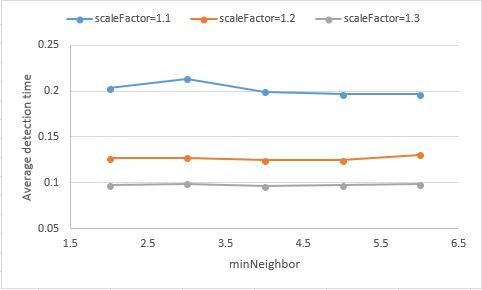
\includegraphics[height=7cm]{chap2/4.jpg}
	\bicaption{scaleFactor与minNeighbor参数对于处理速度的影响}{How parameter scaleFactor and minNeighbor affects processing speed}
	\label{fig:haartest:speed}
\end{figure}

\subsubsection{准确率}

HAAR级联分类器在CFDDB上检测率最高尚未超过$50\%$,没有达到本系统的需求。经过分析,共有两种原因影响了HAAR分类器在CFDDB上的检测效果:

\begin{figure}[!htp]
	\centering
	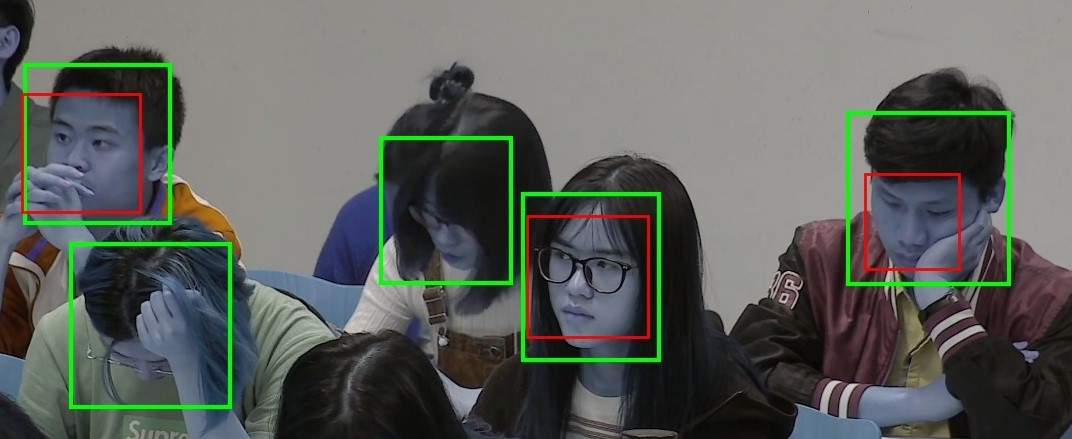
\includegraphics[height=4cm]{chap2/5.jpg}
	\bicaption{有角度和被遮挡的人脸识别结果示例}{Example of angled faces and partially blocked faces}
	\label{fig:haartest:acc}
\end{figure}

第一,HAAR分类器是针对正脸训练的,对侧脸和被遮挡人脸的检测效果非常差。我们将检测结果可视化之后取其中的一张图片分析,如图\ref{fig:haartest:acc}所示。红色的矩形框是HAAR分类器检测到的人脸区域,绿色的矩形框是人工标注的人脸区域。可以看到,只要人脸的角度过大,或者被其他人或物体遮挡,HAAR分类器的检测效果就会大打折扣。

第二,由于HAAR分类器对边缘信息特别敏感,使得在有些情况下会产生错误的识别结果,当minNeighbor=2并且scaleFactor=1.1时,如图\ref{fig:haartest:acc2}所示,HAAR分类器经常会将衣服的褶皱误识别为人脸,将特殊的边缘识别成人脸。

\begin{figure}[!htp]
	\centering
	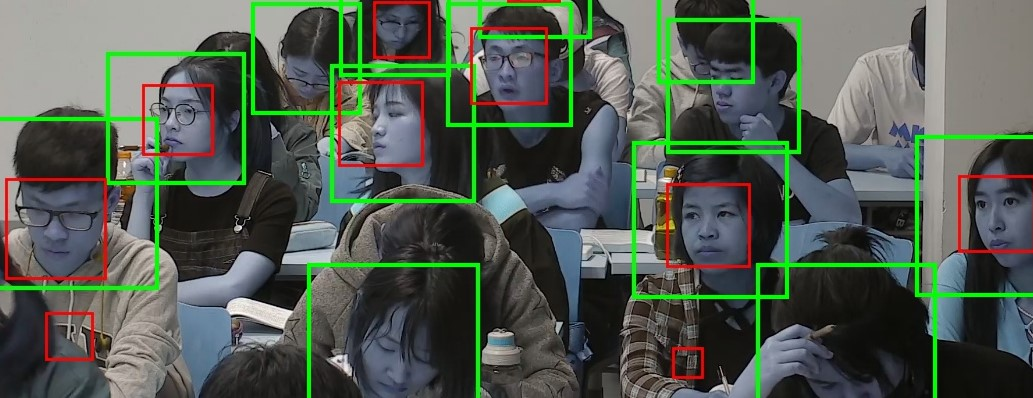
\includegraphics[height=4cm]{chap2/6.jpg}
	\bicaption{HAAR分类器误识别示例}{Haar cascade classifier misidentification example}
	\label{fig:haartest:acc2}
\end{figure}

综上所述,基于HAAR特征的级联分类器存在诸多限制,准确率难以达到要求,并不适合作为本系统的人脸检测模块使用。


\section{MtCNN}

\subsection{概述}

传统的人脸识别方法大多是基于某种分类器从图像中提取特征,根据特征或者特征组合来判断某一图像区域是否属于人脸。然而就像上文所述的HAAR级联分类器,传统的人脸识别的方法往往无法胜任从监控录像所拍摄的图像中提取多个人脸的工作。因此,我们将目光投向了深度学习的方法。

近年来,以卷积神经网络为代表的深度神经网络在计算机视觉的各个领域都有了丰硕的成果,人脸检测也不例外。下面我们就将介绍一种利用深度神经网络执行人脸检测和校正的网络:MtCNN。

MtCNN的全称是多任务级联卷积网络。由Kaipeng Zhang[11]等人中提出。这个网络一经提出就被广泛应用在多种人脸识别的神经网络的训练和测试输入中,是目前广泛应用的人脸检测网络之一。

在MtCNN之前,也有学者尝试使用卷积神经网络进行人脸检测。然而由于他们所使用的卷积神经网络过于复杂,导致计算的时间复杂度极高,无法实用[12]。MtCNN不仅大大提升了人脸检测的速度,而且创造性的将人脸检测和人脸校正合二为一,丰富了网络的功能,为下一步的识别系统提供了极大的方便。

\subsection{总体架构}

MtCNN中共包括三个不同的网络,总体的架构图\ref{fig:mtcnn}所示:

\begin{figure}[!htp]
	\centering
	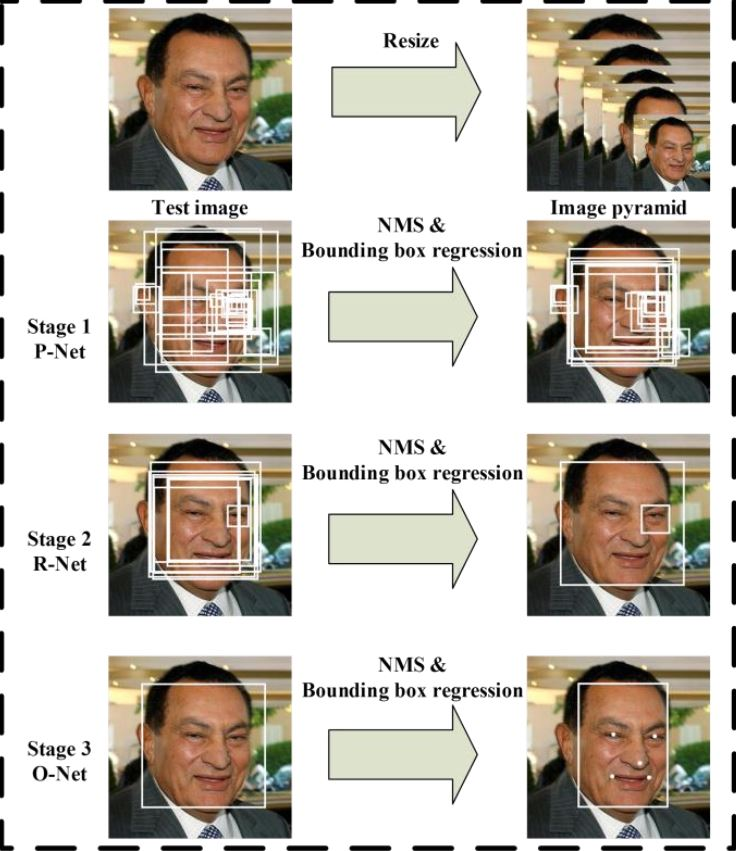
\includegraphics[height=7cm]{chap2/7.jpg}
	\bicaption{MtCNN 总体架构图[11]}{MtCNN overall pipeline}
	\label{fig:mtcnn}
\end{figure}

在接收到一张图片之后,首先将其缩放得到图片金字塔。所得到的图像金字塔是三个级联卷积网络的输入。

第一阶段,我们使用一种全卷积网络叫做Proposal Network(P-Net)来获得候选人脸区域和它们的边界框回归向量[11]。接着使用边界框回归向量去校准候选区域。最后使用非极大值抑制(NMS)整合高度重合的区域。

第二阶段,我们使用另一种卷积网络叫做Refine Network(R-Net)来进一步筛选得到的区域[11]。在筛选结束之后,与第一阶段相同,使用边界框回归对人脸边界进行进一步校准。最后使用NMS整合重合区域。

第三阶段与第二阶段基本相似,但是在这一阶段我们主要对脸部更精细的特征进行描述[11]。这一阶段使用Output Network(O-Net)得到人脸区域的五个特征点。

\subsection{Loss函数设计}

对于每一个样本$x_i$,人脸区域区分部分的Loss函数 其中$p_i$是网络输出结果是人脸区域的概率,$y_i^{det}\in\{0,1\}$是该区域是否是人脸的标签[11]。
\begin{displaymath}
	L_{i}^{det}=-((y_{i}^{det}log(p_{i}))+(1-y_{i}^{det})(1-log(p_i)))
\end{displaymath}



边界框回归的Loss函数 其中$\hat{y}_i^{box}$是由网络得出的结果,$y_i^{box}$是实际的边界框。
\begin{displaymath}
	L_{i}^{box}=||{\hat{y}_i^{box}-y_i^{box}}||_2^2
\end{displaymath}



脸部特征回归的Loss函数 与边界框类似,使用了Euclidean Loss。
\begin{displaymath}
L_{i}^{landmark}=||{\hat{y}_i^{landmark}-y_i^{landmark}}||_2^2
\end{displaymath}



\subsection{在CFDDB上的测试结果}

我们使用预训练完成的MtCNN在CFDDB上进行测试,测试中使用了TensorFlow 1.7.1版本,并使用GPU加速网络运算。测试结果如表\ref{tab:mtcnn}所示,其中confidence表示所取MtCNN输出的人脸区域信任率,averageTime表示平均处理一张图片所需要的时间。

\begin{table}[!hpb]
	\centering
	\bicaption[MtCNN在CFDDB上的测试结果]
	{MtCNN在CFDDB上的测试结果}
	{MtCNN test results on CFDDB}
	\label{tab:mtcnn}
	\begin{tabular}{ cccc | c }
		\hline
		confidence & faceDetected & faceRight & averageTime & recall\\
		\hline
		0.90 & 433 & 388 & 344.38ms & $35.69\%$\\
		0.80 & 465 & 410 & 325.71ms & $37.71\%$\\
		0.70 & 483 & 423 & 357.41ms & $38.91\%$\\
		0.60 & 483 & 423 & 333.66ms & $38.91\%$\\
		\hline
	\end{tabular}
\end{table}

\subsection{结果分析}

\subsubsection{处理速度}

不同的confidence参数处理时间基本一致,均为350ms左右的时间处理一张宽1600像素,高1200像素的图片。由于使用了GPU加速运算,并且将原有的Matlab平台的代码成功移植到了更先进的TensorFlow平台[13],MtCNN处理速度符合我们的要求。

\subsubsection{准确率}

在CFDDB测试集中,MtCNN最多正确检测出了423个人脸区域,检测率最高为$38.91\%$,识别率较低,无法符合我们的要求。但是根据论文[11]在WiderFace中最难的测试集上,MtCNN都有着超过$60\%$的召回率,然而在CFDDB上却无法体现。经过分析,可能的原因有以下两条:

\begin{figure}[!htp]
	\centering
	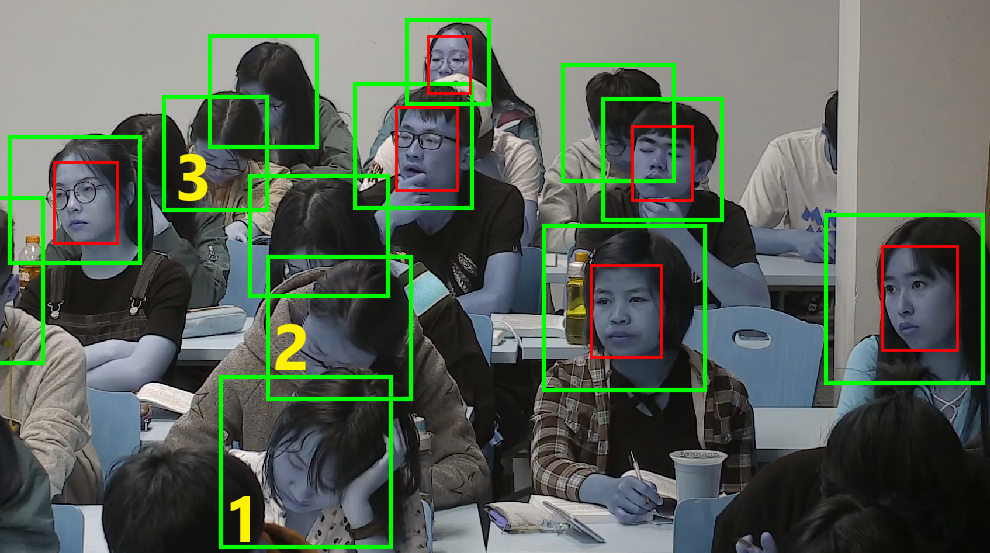
\includegraphics[height=5cm]{chap2/8.png}
	\bicaption{MtCNN 识别结果可视化样例}{MtCNN detect results example}
	\label{fig:mtcnn:accr}
\end{figure}


原因一:对侧脸的识别,五个特征点不完整的人脸识别率较低。CFDDB中有大量侧脸和不完整人脸,如图\ref{fig:mtcnn:accr}所示,其中人脸1俯仰左右都有较大的角度,难以识别;人脸2部分被遮挡,无法提取完整的五个特征点,因此被舍弃;人脸3俯仰角度过大,难以识别。


原因二:CFDDB数据分布的问题,由于数据中样本采集采用的从连续的视频中截取帧的方法,前后两次截取得到的图片差距不大,这样容易导致前一张图片中识别不出的图像往往在下一张图像中一样难以识别。这个问题需要通过扩充CFDDB的样本规模,去除相似度高的图像来解决。

\section{SSH检测器}

\subsection{概述}
SSH的全称为Single Stage Headless face detector,由Mahyar等人提出[14]。SSH检测器针对小脸进行了优化,对处于自然环境的人脸识别有着非常好的效果。在WIDER FACE Hard测试集的测试中,SSH检测器的召回率达到了0.844[14],从检测效果来看,更加符合我们这个系统的需求。

与其他同样基于CNN的人脸检测器相比SSH检测器有如下四个特点:

首先,大多数基于CNN的人脸检测器只针对一种特定大小的人脸进行了训练。因此,在使用的时候需要先建立图像金字塔,然后对图像金字塔中的每一张图片在训练好的网络中前向传播,合并所有前向传播的输出得到结果。而SSH检测器设计了针对三种不同大小人脸的检测器,从不同的网络层中提取信息,使得SSH检测器在使用的时候只需要一次前向传播就可以完成所有大小的人脸检测而无需建立图像金字塔。

其次,大多数基于CNN的人脸检测器将人脸分为两个阶段。第一阶段,浅层的卷积特征图产生候选边界框集合。第二阶段,剩余的分类网络用于从集合中提取局部特征并将其分类。在这样的设计中,在第二阶段必须对第一阶段所有产生的候选框进行计算,从而需要极高的计算代价。而SSH检测器在一个阶段同时完成了边界框回归和最后的分类运算,因此计算代价更小。

再次,在达到国际领先的检测水平的同时,SSH检测器舍弃了基础VGG-16网络中含有大量参数的全连接层,使得训练过程更加容易。同时,也使得网络整体变得轻量快速。

最后, SSH检测器针对每个检测模块分别采用了Online hard negative and positive mining[15]的方法进行训练,使得训练得到的模型误报率更低,更加精确。

\subsection{网络结构}

论文[14]中的图\ref{fig:ssh:arc}展示了SSH检测器的总体架构。从图中可以看出,SSH检测器是一个全卷积深度网络,通过在步长分别为8、16和32的特征图上添加如论文[14]中图\ref{fig:ssh:det}所示的检测模块,实现了利用网络定位和区分人脸区域的功能。检测模块则由二元卷积分类器和回归运算模块组成。

\begin{figure}[!htp]
	\centering
	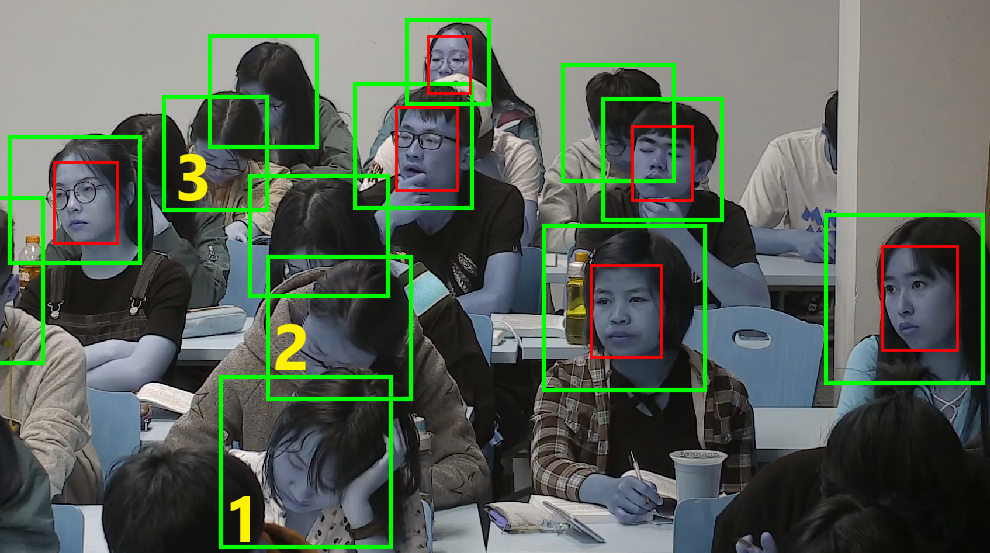
\includegraphics[height=7cm]{chap2/8.jpg}
	\bicaption{SSH 检测器总体架构}{SSH face detector general architecture}
	\label{fig:ssh:arc}
\end{figure}

\begin{figure}[!htp]
	\centering
	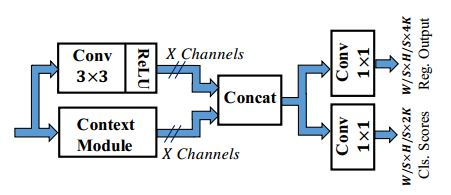
\includegraphics[height=3cm]{chap2/9.jpg}
	\bicaption{SSH 检测模块}{SSH detection module}
	\label{fig:ssh:det}
\end{figure}

\begin{figure}[!htp]
	\centering
	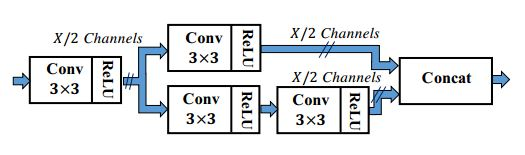
\includegraphics[height=3cm]{chap2/10.jpg}
	\bicaption{SSH 背景环境模块}{SSH context module}
	\label{fig:ssh:context}
\end{figure}

正如SSH检测器概述中所述,SSH检测器为单阶段检测器,并没有产生边界框候选集的阶段。事实上,SSH检测器通过对预先定义的边界框集进行回归而得到人脸区域的。而这个边界框集是通过密集的、重叠的滑动窗口所定义的。

而对于检测模块而言,有一系列的卷积层用于检测人脸的面部特征和位置定位,其中就包括了一个背景环境模块,如论文[14]中图\ref{fig:ssh:context}。这个背景环境模块用于提高感受野的有效性,从而提高网络的检测精度。背景环境在人脸较小或者不清晰的时候可以向检测器提供非常重要的信息。因为当人脸面部信息被遮挡或者不清晰的时候,人脸周围的背景环境例如衣领、头发等信息可以作为面部区域的关键的辅助信息传入网络中,帮助网络断定这个区域是否为人脸区域。

事实上,在另一个由Peiyun Hu等人提出的小脸检测器的论文中[17]详细叙述了背景区域对于小脸检测的重要性。根据论文中的叙述,增加背景环境信息几乎总是有效的,无论对于大脸还是小脸。作者在实验中发现唯一降低了识别准确率的情况是向宽25像素,高25像素的小脸区域加入了超过宽300像素,高300像素的背景信息区域。而这种情况识别率降低的主要原因是向感受野中加入了明显过多的背景信息而导致了检测器发生了过拟合现象。


\subsection{在CFDDB上的测试结果}

我们使用预训练完成的SSH检测器在CFDDB上进行测试,测试中使用了GPU加速网络运算。测试结果如表\ref{tab:ssh}所示,其中confidence表示所取SSH检测器输出的人脸区域信任率,averageTime表示平均处理一张图片所需要的时间。

\begin{table}[!hpb]
	\centering
	\bicaption[SSH检测器在CFDDB上的测试结果]
	{SSH在CFDDB上的测试结果}
	{SSH test results on CFDDB}
	\label{tab:ssh}
	\begin{tabular}{ cccc | c }
		\hline
		confidence & faceDetected & faceRight & averageTime & recall\\
		\hline
		0.90 & 921 & 915 & 228.37ms & $85.10\%$\\
		0.80 & 957 & 950 & 227.76ms & $87.39\%$\\
		0.70 & 975 & 966 & 226.67ms & $88.87\%$\\
		0.60 & 989 & 980 & 229.27ms & $90.16\%$\\
		0.50 & 1008 & 998 & 230.43ms & $91.81\%$\\
		\hline
	\end{tabular}
\end{table}

\subsection{结果分析}

\subsubsection{处理速度}

不同的confidence参数处理时间基本一致,均为230ms左右的时间处理一张宽1600像素,高1200像素的图片。由于使用了GPU加速运算,而且SSH检测器使用了轻量级的网络,使得处理时间完全满足系统需求。

\subsubsection{准确率}

在CFDDB测试集中,SSH检测器最多正确检测出了998个人脸区域,识别率高达$91.81\%$。即使将confidence参数调高至0.9,识别率任然达到了$85.1\%$,超过了$80\%$的要求。因此,SSH检测器的准确率也完全可以满足系统的需求,适合作为人脸检测模块的核心算法。

\subsection{网络优化与平台移植}

虽然SSH检测满足了我们的检测条件,但是我们在测试中也发现了SSH存在的一些待改进的问题。

首先,SSH检测器目前只有Caffe平台的实现,这对于测试和部署都是一项极大的挑战。Caffe平台虽然功能强大,但是搭建GPU支持的Caffe环境却必须从源码进行编译。这就意味和每次部署搭建环境时都必须安装数量庞大的依赖库,并下载源码编译。整个过程需要耗费大量的时间,不利于规模性部署。而且随着Caffe平台的维护力度逐渐减小,最新版本的显卡驱动和深度神经网络加速库均无法使用,使得网络的运行效率下降。同时,Caffe平台对于嵌入式设备的支持优化较少,不利于将识别模块移植到嵌入式平台上使用。

其次,SSH检测器基于性能较弱的VGG-16网络改进而来,存在提升的空间。如果将其中的VGG-16网络替换为对应的MobileNets网络[18],或者MobileNetsV2网络[19],则不仅可以提升网络的运行速度,而且更方便将网络移植到嵌入式设备等没有GPU支持的设备中使用。

最后,SSH检测器难以兼容使用TensorFlow实现的人脸识别算法。由于Caffe平台和TensorFlow平台使用了不同版本的Protocol Buffer依赖库,如果希望能够同时运行两个平台就需要安装老旧版本的TensorFlow平台并进行一些繁琐的设置。这不仅损失了人脸识别算法的运行效率,而且给规模化部署带来了更多的挑战。

\section{Tiny face检测器}

\subsection{概述}

Tiny face检测器,是由Peiyun Hu等人在论文[17]中提出的一种针对小脸进行优化处理的人脸检测器,也是最早针对小脸进行检测的深度网络之一。Tiny face使用了图像金字塔和多种不同大小、不同宽高比的模板来检测不同大小人脸,并基于VGG-16[]网络,ResNet-101[]和ResNet-50网络结构都进行了实现。其中基于ResNet-101的实现在WiderFace测试集Hard部分的召回率达到了0.823。

经过SSH


\subsection{在CFDDB上的测试结果}

\begin{table}[!hpb]
	\centering
	\bicaption[Tiny face检测器在CFDDB上的测试结果]
	{Tiny face检测器在CFDDB上的测试结果}
	{Tiny face detector test results on CFDDB}
	\label{tab:tiny}
	\begin{tabular}{ cccc | c }
		\hline
		confidence & faceDetected & faceRight & averageTime & recall\\
		\hline
		0.90 & 921 & 915 & 228.37ms & $85.10\%$\\
		0.80 & 957 & 950 & 227.76ms & $87.39\%$\\
		0.70 & 975 & 966 & 226.67ms & $88.87\%$\\
		0.60 & 989 & 980 & 229.27ms & $90.16\%$\\
		0.50 & 1008 & 998 & 230.43ms & $91.81\%$\\
		\hline
	\end{tabular}
\end{table}

